\documentclass[6008notes.tex]{subfiles}
\begin{document}
\graphicspath{ {images/intropl/} }

\section{Introduction to Learning Probabilistic Models}

As we have seen, graphical models are a powerful mechanism for capturing structure in distributions that enables efficient inference. We're now ready to talk about how to choose such models. This is the problem of model selection. Invariably, domain knowledge guides aspects of the model we choose -- for example, the underlying physics, biology, economics, et cetera. However, in practice, some aspects of the model we must often learn directly from data.

So now let's turn our attention to how to learn models. We'll begin with a discussion of a rather general framework of learning based on the time-honored principle of maximum likelihood. We will then put it to work to help us learn a wide range of tree-structured graphical models, including hidden Markov models and what are referred to as naive Bayes models -- which, despite their name, are surprisingly powerful.

In particular, we'll show how to efficiently learn the conditional distribution tables that characterize a tree model. This is called parameter estimation. And we will see that the concept of empirical distributions or histograms plays an important role.

Finally, we will show how to solve the problem of finding a tree that best fits the data, which is referred to as structure learning. Amazingly, even though there are a super exponential number of possible trees, we will see how to solve the problem with only quadratic search complexity using the celebrated Chow-Liu algorithm, which is based on measuring empirical mutual information. Exciting applications for the learning methodology we develop are everywhere, from natural language processing and automatic face recognition to phylogenetics and well beyond. So let's begin.

\subsection{Learning Probabilistic Models: Notation and Outline}

Thus far in the course, we've been given a probabilistic model of the uncertain world, from which we produced predictions given observations. But where do these probabilistic models come from? We now turn to the problem of learning such models (also referred to as model selection since we are selecting which model to use).

As a concrete example that we'll build on later in this section: We don't actually know the underlying probability distribution for what makes an email considered spam vs. ``ham'' (i.e., not spam). However, we do have access to plenty of training examples of what emails are spam or ham, where a user has manually flagged her or his incoming emails as spam or not. From all these training examples, we could learn a model for what spam emails look like and what ham emails look like.

There are two levels of learning we consider:

\begin{itemize}
\item Parameter learning: Suppose we know what the edges are in an undirected graphical model but we don't know what the table entries should be for the potentials -- how do we estimate these entries?

\item Structure learning: What if we know neither the parameters nor which edges are present in an undirected graphical model? In this case, we could first figure out what edges are present. After we decide on which edges are present, then the problem reduces to the first problem of parameter learning.
\end{itemize}

In both cases, the high-level setup is the same: there is some underlying probability distribution $p$ that we don't know details for but want to learn. The distribution $p$ has some parameter (or a set of parameters) $\theta$. We will assume that we can collect $n$ independent samples $X^{(1)}, \dots , X^{(n)}$ from the distribution $p$ (these $n$ samples are often referred to as ``training data''). Given these samples, we aim to estimate $\theta$ using what's called ``maximum likelihood'', which tries to learn a model that in some sense best fits the training data we have available. Along the way, we will see how information theory plays a crucial role in helping us not only develop computer programs to learn probability distributions but it also provides an interpretation of what the programs are doing.

We begin with parameter learning, starting with a single node graphical model and working our way to richer graphical models whose potential table entries we aim to learn:

\begin{enumerate}
\item A single node undirected graphical model corresponding to a single finite random variable

\item A graphical model called the naive Bayes model which can be used for tasks like email spam detection and handwritten digit recognition

\item General tree-structured undirected graphical models
\end{enumerate}

We then turn toward structure learning, proceeding directly to the most general class of graphical models we consider: tree-structured undirected graphical models, where we learn which edges to include in the tree and what potential tables to assign to the edges.

\section{Introduction to Parameter Learning - Maximum Likelihood and MAP Estimation }

\subsection{Introduction to Maximum Likelihood}

We consider a single binary random variable $X$, that for simplicity can be thought of as a (possibly biased) coin flip, taking on values in the set $\mathcal{X}=\{ \text {heads},\text {tails}\}$. While this setup is extremely simple, understanding how parameter learning works here will already give us most of the intuition for our parameter learning coverage! We'll generalize to the finite (can be non-binary) random variable case later.

The issue is that the probability of heads, which denote $\theta$, is unknown, and we'd like to estimate (or ``learn'') this probability.

The probability table is:

{\centering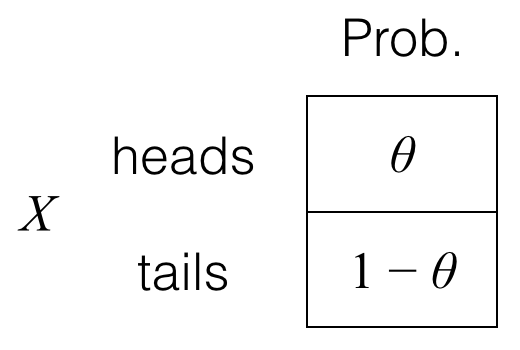
\includegraphics[scale=0.4]{images_sec-maximum-likelihood-intro} \par}

\textbf{Notation:} Recall that previously we would write the probability table of random variable $X$ as $p_X$ or $p_X(\cdot)$. However, now to make it explicit that we don't know $\theta$, which we aim to estimate, we will denote the probability table as $p_{X}(\cdot ;\theta )$. The semi-colon is used to say that everything after the semi-colon in the parentheses refers to parameter(s) of the model. The probability that $X=x$ is denoted as $p_{X}(\cdot ;\theta )$.

To estimate parameter $\theta$, we assume we have flipped the coin n times to get outcomes $X^{(1)},X^{(2)},\dots ,X^{(n)}$ which are i.i.d. samples from the same distribution as $X$. In other words,

{\centering$p_{X^{(1)},X^{(2)},\dots ,X^{(n)}}(x^{(1)},x^{(2)},\dots ,x^{(n)};\theta )=\prod _{i=1}^{n}p_{X}(x^{(i)};\theta ).$ \par}
 
The above probability is called the ``likelihood'' of the data -- it is the probability of seeing the observed data as a function of the unknown parameter $theta$. Note that the observed data are treated as fixed constants! We denote the likelihood as $L(\theta)$.

As an example, if we observed the sequence heads, tails, heads, then $n=3$, $X^{(1)} = \text {heads}$, $X^{(2)} = \text {tails}$, and $X^{(3)} = \text {heads}$, and the likelihood is

{\centering$L(\theta ) = \underbrace{\theta }_{\text {heads}} \cdot \underbrace{(1 - \theta )}_{\text {tails}} \cdot \underbrace{\theta }_{\text {heads}} = \theta ^2 (1 - \theta ).$ \par}
 
Next, to estimate (or learn) $\theta$, we will use ``maximum likelihood'' which maximizes the likelihood function $L$ over possible values of the parameter $\theta$. Put another way, we find whichever probability of heads $\theta$ makes the probability of seeing the samples $X^{(1)}=x^{(1)},X^{(2)}=x^{(2)},\dots ,X^{(n)}=x^{(n)}$ as high as possible.

Formally, the maximum likelihood estimate $\widehat{\theta }$ for parameter $\theta$ is the solution to the following optimization problem:

{\centering$\widehat{\theta }=\arg \max _{\theta \in [0,1]}\underbrace{\prod _{i=1}^{n}p_{X}(x^{(i)};\theta )}_{\text {likelihood}}.$ \par}
 
It turns out the answer in this case is quite simple.

\textbf{Claim:} The maximum likelihood estimate $\widehat{\theta }$ for the true probability of heads $\theta$ is simply the fraction of times we see heads in the observed sequence $x^{(1)},\dots ,x^{(n)}$, i.e.,

{\centering$\widehat{\theta }=\frac{\text {number of times heads appears}}{n}=\frac{\sum _{i=1}^{n}\mathbf{1}\{ x^{(i)}=\text {heads}\} }{n}.$ \par}
 
For example, if we observed the sequence heads, tails, heads, then the maximum likelihood estimate for the probability of heads is 2/3 since 2/3 of the tosses were heads.

Let's prove the claim.

First, by how the problem is set up:

{\centering$p_{X}(x^{(i)};\theta)=\begin{cases}
\theta & \text{if }x^{(i)}=\text{heads},\\
1-\theta & \text{if }x^{(i)}=\text{tails}.
\end{cases}$ \par}

Next, letting $n_{\text {heads}}\triangleq \sum _{i=1}^{n}\mathbf{1}\{ x^{(i)}=\text {heads}\}$ be the number of times heads occurred, and $n_{\text {tails}}\triangleq \sum _{i=1}^{n}\mathbf{1}\{ x^{(i)}=\text {tails}\}$ be the number of times tails occurred, we have, due to independence of the coin flips and because the coin flips all have the same distribution:

\begin{eqnarray*}
% \text{likelihood}
L(\theta)
&=& \prod_{i=1}^{n}p_{X}(x^{(i)};\theta) \\
&=& \big(\underbrace{\theta\times\cdots\times\theta}_{n_{\text{heads}}\text{ times}}\big)\times\big(\underbrace{(1-\theta)\times\cdots\times(1-\theta)}_{n_{\text{tails}}\text{ times}}\big) \\
&=& \theta^{n_{\text{heads}}}(1-\theta)^{n_{\text{tails}}}.
\end{eqnarray*}

Our next goal is to maximize the likelihood. Mathematically it'll be easier to work with the log of the likelihood. Note that the value of $\theta$ that maximizes the likelihood is the same as the value of $\theta$ that maximizes the log of the likelihood, because the log function is strictly increasing, so:

\begin{eqnarray*}
\widehat{\theta} &=&\arg\max_{\theta\in[0,1]} L(\theta) \\
&=&\arg\max_{\theta\in[0,1]}\log( L(\theta) )\\
&=&\arg\max_{\theta\in[0,1]}\log\big(\theta^{n_{\text{heads}}}(1-\theta)^{n_{\text{tails}}}\big)\\
&=&\arg\max_{\theta\in[0,1]}\big\{\underbrace{n_{\text{heads}}\log\theta+n_{\text{tails}}\log(1-\theta)}_{\triangleq\ell(\theta)}\big\}.
\end{eqnarray*}

Let's examine the log likelihood function $\ell$ that we've just defined and that we're aiming to maximize:

{\centering$\ell (\theta )=n_{\text {heads}}\log \theta +n_{\text {tails}}\log (1-\theta ).$ \par}
 
From calculus you may remember that we can optimize this function by looking at what value for $\theta$ makes $\frac{d\ell (\theta )}{d\theta }=0$. It turns out that this will be sufficient and solving this optimization (which we'll spell out shortly) will yield that the optimal $\widehat{\theta }$ is the fraction of heads observed in the $n$ flips.

However, for just this binary random variable case, we'll be a little bit more rigorous and give all the details, which should help you connect what you've seen in calculus to what is happening here in maximum likelihood estimation.

Without further ado, when we maximize $\ell (\theta )$, we break the problem up into three cases:

\begin{itemize}
\item If $n_{\text {tails}}=0$, then

{\centering$\ell (\theta )=n_{\text {heads}}\log \theta$ \par}
 
is maximized when $\theta=1$ since $\log \theta$ increases as $\theta$ ranges from 0 to 1.

\item If $n_{\text {heads}}=0$, then

{\centering$\ell (\theta )=n_{\text {tails}}\log (1-\theta )$ \par}
 
is maximized when $\theta=0$ since $\log (1-\theta )$ decreases as we increase $\theta$ from 0 to 1.

\item If neither $n_{\text {heads}}$ nor $n_{\text {tails}}$ is 0, which means that both are positive (they can't be negative, and they can't both be 0 since that would mean we didn't have any observations), then note that $\ell$ is a differentiable real-valued function defined on the domain $0< \theta <1$. To see why this is the case:

\begin{itemize}
\item Note that we can't have $\theta<0$ or $\theta>1$ because in both of these cases, we'd have a term in $\ell (\theta )$ that is the log of a negative number, which isn't defined for real-valued functions.

\item When $\theta=0$ or $\theta=1$, we encounter a term $\log 0=-\infty$, which is not a real number, and so $\ell (\theta )$ in this case is not a real number.

\item When $\theta \in (0,1)$, then $\log \theta$ and $\log (1-\theta )$ are both real numbers, and so is $\ell (\theta )$.
\end{itemize}
\end{itemize}

Thus, $\ell$ is only a real-valued function on the interval $\theta \in (0,1)$. In fact, within this interval, we can compute its first and second derivatives (which we'll do shortly). At this point we recall from calculus that to optimize $\ell$, it's sufficient to do two steps:

\begin{enumerate}
\item Find when $\frac{d\ell (\theta )}{d\theta }=0$. Supposing that this happens for only one value of $\theta$, we'll call this best value $\widehat{\theta }$.

\item Check that the second derivative $\frac{d^{2}\ell }{d\theta ^{2}}$ evaluated at $\widehat{\theta }$ is negative, which implies that the point we found in the first step corresponds to the unique maximum.
\end{enumerate}

Let's do step 1:

\begin{eqnarray*}
0&=&\Big[\frac{d\ell}{d\theta}\Big]_{\theta=\widehat{\theta}}\\
 &=&\bigg[\frac{d}{d\theta}\big\{ n_{\text{heads}}\log\theta+n_{\text{tails}}\log(1-\theta)\big\}\bigg]_{\theta=\widehat{\theta}}\\
&=&\bigg[n_{\text{heads}}\frac{1}{\theta}-n_{\text{tails}}\frac{1}{1-\theta}\bigg]_{\theta=\widehat{\theta}}\\
&=&n_{\text{heads}}\frac{1}{\widehat{\theta}}-n_{\text{tails}}\frac{1}{1-\widehat{\theta}}.
\end{eqnarray*}

Multiplying through by $\widehat{\theta }(1-\widehat{\theta })$, we get:

\begin{eqnarray*}
0
&=& n_{\text{heads}}(1-\widehat{\theta})-n_{\text{tails}}\widehat{\theta} \\
&=& n_{\text{heads}}-n_{\text{heads}}\widehat{\theta}-n_{\text{tails}}\widehat{\theta} \\
&=& n_{\text{heads}}-(n_{\text{heads}}+n_{\text{tails}})\widehat{\theta}.
\end{eqnarray*}

In other words,

{\centering$\widehat{\theta }=\frac{n_{\text {heads}}}{n_{\text {heads}}+n_{\text {tails}}}=\frac{n_{\text {heads}}}{n}. $ \par}
 
Step 2: The second derivative of $\ell$ with respective to $\theta$ is

{\centering$\frac{d^{2}\ell }{d\theta ^{2}}=-n_{\text {heads}}\frac{1}{\theta ^{2}}-n_{\text {tails}}\frac{1}{(1-\theta )^{2}},$ \par}
 
which is always negative since $\theta^2$ and $(1-\theta )^{2}$ are always positive when $\theta \in (0,1)$.

Lastly, we also check the boundary, i.e., we make sure that indeed the log likelihood $\ell$ evaluated at $\widehat{\theta}$ is larger than each of $\ell(0)$ and $\ell(1)$. We have

{\centering{\renewcommand{\arraystretch}{1.5}
\begin{tabular}{l l l}
$\ell (0)$ & $=$ & $\underbrace{n_{\text {heads}} \log 0}_{-\infty } + \underbrace{n_{\text {tails}} \log 1}_0 = -\infty ,$ \\
$\ell (1)$ & $=$ & $\underbrace{n_{\text {heads}} \log 1}_0 + \underbrace{n_{\text {tails}} \log 0}_{-\infty } = -\infty ,$ \\
$\ell (\widehat{\theta })$ & $=$ & $n_{\text {heads}} \underbrace{\log \frac{n_{\text {heads}}}n}_{>-\infty } + n_{\text {tails}} \underbrace{\log \frac{n_{\text {tails}}}n}_{>-\infty } > -\infty ,$ 
\end{tabular}} \par}
	
so indeed $\ell (\widehat{\theta }) > \ell (0)$ and $\ell (\widehat{\theta }) > \ell (1)$.

To summarize:

\begin{itemize}
\item If $n_{\text {tails}}=0$, then we set $\widehat{\theta }=1$

\item If $n_{\text {heads}}=0$, then we set $\widehat{\theta }=0$

\item If $n_{\text {heads}}>0$ and $n_{\text {tails}}=0$, then we set 

{\centering$\widehat{\theta }=\frac{n_{\text {heads}}}{n},$ \par}
 
from which we see that this same formula holds true even for the cases of $n_{\text {tails}}=0$ or $n_{\text {heads}}=0$. The only reason why we were careful to look at the first two cases separately is because the log likelihood function $\ell$ is neither real-valued nor differentiable at $\theta=0$ or $\theta=1$, corresponding to the $n_{\text {heads}}=0$ and $n_{\text {tails}}=0$ cases.
\end{itemize}

Putting together the pieces, the maximum likelihood estimate for the probability of heads is equal to the fraction of heads we see amongst our $n$ coin flips:

{\centering$\widehat{\theta }=\frac{n_{\text {heads}}}{n}.$ \par}
 
\textbf{Remark:} If we didn't take the log, we could still proceed with the same calculus tools but immediately the derivatives get messy due to the product rule of derivatives! Note though that it's not always the case that taking the log makes sense, as you'll see in one of the problems.


\subsection{Practice Problem: The German Tank Problem}

Suppose the Germans have $k$ tanks, numbered $1, \,  2, \,  \dots , \,  k$. The Allies observe $n<k$ tanks with numbers $x^{(1)}, \,  x^{(2)}, \,  \dots , \,  x^{(n)}$. Assume that these numbers are drawn uniformly without replacement from $\{ 1, \,  2, \,  \dots , \,  k \}$. The objective is to get an estimate $\widehat{k}$ of the total number of German tanks.

\begin{itemize}
\item \textbf{(a)} What is the ML estimate for $k$?

Hints: Keep in mind that each $x^{(i)}$ is a value in $\{ 1, \,  \dots , \,  k \}$. Also, this is one of those maximum likelihood problems where taking the log isn't helpful.

\item \textbf{(b)} What is the bias of the ML estimate $\widehat{k}_{\text {ML}}(X^{(1)},\dots ,X^{(n)})$ for $k$?

\item \textbf{(b)} Determine an unbiased estimator for $k$ based on the maximum likelihood estimate $\widehat{k}_{\text {ML}}$ for $k$.
\end{itemize}

Hint: Start by using your answer from (b) and setting the bias equal to 0 and solving for $k$.

\paragraph{Solutions}

\textbf{(a)} There are ${k \choose n}$ possible choices of which tanks we observe. Each of these is equally likely, so the likelihood is

{\centering$p_ X(x; \theta ) = \frac{\mathbf{1}\{ 1\le x^{(1)} \le k, 1 \le x^{(2)} \le k, \dots , 1 \le x^{(n)} \le k\} }{{k \choose n}}.$ \par}
 
The numerator says that each $x^{(i)}$ (i.e., the number the tank is labeled with) must be between 1 and $k$, the maximum number.

Now notice that with $n$ treated as fixed, then to maximize the likelihood, we want the denominator to be as small as possible, which means that we want $k$ to be as small as possible. However, the smallest $k$ can be so that the numerator is nonzero is when $k = \max (x^{(1)}, \dots , x^{(n)})$. Thus, the ML estimator for $k$ is given by

{\centering$\widehat{k}_{\text {ML}} = \max (x^{(1)}, \dots , x^{(n)}).$ \par}

\textbf{(b)} We want to evaluate the expectation of

{\centering$\widehat{k}_\text {ML}(X^{(1)},\dots ,X^{(n)}) = \max (X^{(1)},X^{(2)},\dots ,X^{(n)}).$ \par}
 
The probability that the maximum tank number/label observed is $m$ is $\frac{\binom {k-1}{n-1}}{\binom {k}{n}}$ since there are $\binom {k}{n}$ possible ways to observe $n$ tanks, and $\binom {m-1}{n-1}$ ways in which we definitely picked the tank with number $m$ and among the tanks with smaller numbers (i.e., among $m-1$ tanks) we choose $n-1$ of them. Then

{\centering$\mathbb {E}[\widehat{k}_\text {ML}(X^{(1)},\dots ,X^{(n)})] = \sum _{m=n}^{k} m \mathbb {P}(\text {max number observed is }m) = \sum _{m=n}^{k} m \frac{ \binom {m-1}{n-1}}{ \binom {k}{n}} = \frac{n (k+1)}{n+1},$ \par}
 
where in the last step, we evaluate the expression using a calculator. Thus, the bias of the ML estimator for k in this case is

{\centering$\mathbb {E}[\widehat{k}_\text {ML}(X^{(1)},\dots ,X^{(n)})] = \sum _{m=n}^{k} m \mathbb {P}(\text {max number observed is }m) = \sum _{m=n}^{k} m \frac{ \binom {m-1}{n-1}}{ \binom {k}{n}} = \frac{n (k+1)}{n+1},$ \par}
 
where as a reminder, note that $n \le k$. This means that the ML estimator on average guesses a value of $k$ that is lower than the true value. This makes sense since if we just take the maximum of the numbers on the tanks we've seen, then unless we see the tank with number $k$, the maximum we observe is going to be smaller than the true maximum. Of course, if we see all the tanks, i.e., if $n=k$, then we definitely see the tank with max number $k$ so the bias in this case would be 0.

\textbf{(c)} The bias is given by

{\centering$\mathbb {E}[\widehat{k}_{\text {ML}}]-k=\frac{n-k}{n+1}=\frac{n}{n+1}-\frac{k}{n+1}.$ \par}
 
Thus,

{\centering$\mathbb {E}[\widehat{k}_{\text {ML}}]-\frac{n}{n+1}=\underbrace{\Big(1-\frac{1}{n+1}\Big)}_{\frac{n}{n+1}}k.$ \par}
 
So

{\centering$k=\underbrace{\frac{n+1}{n}}_{1+\frac{1}{n}}\mathbb {E}[\widehat{k}_{\text {ML}}]-1.$ \par}
 
Thus, an estimator

{\centering$\widehat{k}=\Big(1+\frac{1}{n}\Big)\widehat{k}_{\text {ML}}-1$ \par}
 
will be unbiased since, by linearity of expectation,

{\centering$\mathbb {E}[\widehat{k}]=\Big(1+\frac{1}{n}\Big)\mathbb {E}[\widehat{k}_{\text {ML}}]-1.$ \par}


\subsection{The Bayesian Approach to Learning Parameters}

TODO -- add notes from video

% For estimating the bias of a coin, we saw in a previous video that the maximum likelihood estimate for the probability of heads was just the fraction of heads that we saw in the training data For example if our training data consisted of the sequence heads, tails, heads then the maximum likelihood estimate for the probability of heads would be 2/3. But you might say, "There are only three tosses! "That's not enough data to claim that the probability of heads is actually 2/3." The coin could still be fair for example. And as another extreme example, if we only see one toss-- for example if we only saw heads. Then the maximum likelihood estimate would be 1 because the fraction of heads is one. Even though there's only one toss! So this video briefly suggests an alternative approach, which is a Bayesian approach to learning parameters. In particular instead of treating the parameter as some fix unknown constant, the Bayesian school of thought instead treats parameter theta as a random variable. So rather than having this semicolon we instead have our earlier notation of conditioning on theta where now theta-- so this is capital Theta-- is a random variable corresponding to the parameter of the distribution. Now we can impose some prior beliefs for what the parameters should be by choosing what the function p of capital Theta is where p of capital Theta of little theta can be thought of as a non-negative weight for how much we prefer this specific choice little theta before observing any training data. As a technical note p theta here is in general not like the probability tables we have seen so far in the course because random variable capital Theta has an alphabet that is the closed interval 0 to 1. This alphabet is neither finite nor countably infinite. Theta is actually what is called a continuous random variable. For the purposes of this video though, you don't need to know the specifics of continuous random variables. Instead it's enough to think of p sub capital Theta of little theta as just a non-negative weight given to a specific parameter choice little theta. So instead of maximizing the likelihood-- so here I'll write theta hat sub ML for maximum likelihood-- Now we'll instead maximize-- we'll have argmax over theta within 0, 1 of the likelihood which I'll now actually write out so it's p of X 1, X 2, X 3 of heads, tails, heads, and then here-- conditioned on parameter capital Theta-- so given theta. So this is the likelihood. Now we'll actually try to maximize the likelihood times the prior on parameter theta given by this function here. So likelihood times prior. And the product rule for random variables actually says that this product here is actually the joint distribution of the training data X 1 up through X 3 in this case, and capital Theta, the parameter. So this is the joint distribution and actually the argmax-- treating the training data here heads, tails, heads as fixed-- the arg max of the joint is the same thing as the argmax of we have this joint again, so let me just copy it down here-- so the joint divided by the probability of just the training data. Heads, tails, heads. Again we're treating the training data we observed as fixed. So this thing here is the posterior. So this is just p of capital Theta given X 1, X 2, and X 3 of little theta given heads, tails, heads. So we're doing an argmax over theta of the posterior. And we've seen this earlier before. This is just theta hat MAP for maximum a posteriori. So I'm now going to show you two examples of this prior and work out what theta hat MAP is. So here's the first example, where we we have p of capital Theta of theta is just going to be given by theta times 1 minus theta, for theta within 0, 1. And so the MAP estimate in this case data theta hat MAP is going to be equal to argmax over theta between 0 and 1 of the likelihood, which is theta squared times 1 minus theta. This comes from there being 2 heads and 1 tails in this heads, tails, heads example that we're still using. So we have the likelihood multiplied by the prior, which is theta times 1 minus theta. So this is of course theta cubed times 1 minus theta squared. And we've already seen how to maximize this-- we take the log and we set the derivative with respect to theta to be equal to 0. But just by pattern matching, note that maximizing this is the same thing as doing an ML estimate when there are 3 heads and 2 tails. So the answer to this argmax is going to just be the fraction of heads where we have 3 heads and 2 tails, which is 3 over 3 plus 2, which is 3 over 5. And one way you can think about this is that here this prior where we have theta times 1 minus theta. This theta is going to introduce a pseudo count of 1 heads, and this 1 minus theta is going to introduce a pseudo count of 1 tails, meaning that if you n H heads and n T tails then what this prior is going to do is actually going to make it seem like there are n H plus 1 heads, and n T plus 1 tails. And then with this many heads and this many tails, it's just going to do the ML estimate for those tosses. So again it's as if we introduce a pseudo count for heads, and a pseudo count for tails, and then just did maximum likelihood estimation. To make that clear I'll give a different example here where we have the prior is given by so now I have this theta to the power of 100 times 1 minus theta to the power of 100 again with the observed sequence heads, tails, heads, The MAP estimate is going to be argmax over theta of the likelihood which is theta squared times 1 minus theta times this theta to the power of 100 times 1 minus theta to the power of 100. And this thing is going to be theta to the power of 102 times 1 minus theta to the power of 101. And so again we've seen how to maximize an expression like this. It is like maximum likelihood, where we have 102 heads and 101 tails. So theta hat MAP in this case is going to be 102 divided by 102 plus 101. So in particular this prior is basically making it look as if we're doing maximum likelihood, except where the number of heads is now the actual number of heads plus 100. So we have a pseudo count of 100 heads that are being introduced and then we have the number of tails appearing like the actual number of tails plus this 100. And so for this particular case in general we would have theta hat MAP being equal to number of heads plus 100 divided by the sum of these two things where n H plus n H is of course n. So we're going to have n plus 200. What this prior here is doing is much more so than the previous prior that we saw when we have this 100 and 100 it's making it so that when the number of observations n is small, we're going to really, really think that the coin is probably fair. So this number down here for example-- this is pretty close to 1/2. So when the number of observations is small we're going to essentially bias our estimate to be close to 100 over 200 because for n H and n small basically the dominating terms are just 100 and 200 so this thing will be close to 1/2. However when we crank up the amount of training data we have n, then eventually when n is large and n H is possibly large than n H and n are going to take over and dominate this 100 over 200. So the high-level idea is that for this Bayesian approach to learning parameters, we can neatly account for how much training data we have where when we don't have that much training data we trust our prior more but when we have tons of training data, then we side with the data more and basically our answer will look more like the ML estimate. So that is MAP estimation for learning parameters.

\subsection{Parameter Learning: What's Next}

The single-variable calculus tools for showing what the maximum likelihood or even what the MAP estimate is are not easily going to generalize when we have a large number of parameters that we want to estimate, especially to justify why a particular estimate is actually the argmax. We will soon turn to deriving maximum likelihood estimates using information theoretic measures. Before heading there though, we will be covering a simple way of doing predictions with what's called the naive Bayes classifier, which you'll be using to build an email spam detector.

\end{document}
